% ============================================================
%  ERA:AI Fellowship Poster — Steering Vectors Differ Across Personas
%  A1 portrait (594 × 841 mm) — manual layout for precise control
% ============================================================
\documentclass[a1paper]{article}

\usepackage[a1paper, margin=15mm, top=12mm, bottom=12mm]{geometry}
\usepackage[T1]{fontenc}
\usepackage{lmodern}
\usepackage{graphicx}
\usepackage{xcolor}
\usepackage{enumitem}
\usepackage{microtype}
\usepackage{amsmath}
\usepackage{multicol}
\usepackage{tcolorbox}
\tcbuselibrary{skins, breakable}
\usepackage{tikz}
\usepackage{calc}
\usepackage{setspace}

\pagestyle{empty}

% ── ERA:AI Colour Palette ──────────────────────────────────
\definecolor{eracrimson}{HTML}{8B1A1A}
\definecolor{eradark}{HTML}{6B1010}
\definecolor{eracharcoal}{HTML}{2C2C2C}
\definecolor{eralightgrey}{HTML}{F3F3F3}
\definecolor{erawhite}{HTML}{FFFFFF}
\definecolor{erahighlight}{HTML}{FDF2F2}

% ── Font sizes for A1 readability ──────────────────────────
% Title: ~60pt, Section heads: ~36pt, Body: ~24pt
\newcommand{\postertitle}[1]{{\fontsize{60}{66}\selectfont\bfseries\color{white}#1}}
\newcommand{\posterauthor}[1]{{\fontsize{28}{34}\selectfont\color{white!85}#1}}
\newcommand{\posterinst}[1]{{\fontsize{24}{30}\selectfont\color{white!70}#1}}
\newcommand{\sectionhead}[1]{{\fontsize{34}{40}\selectfont\bfseries\color{white}#1}}
\newcommand{\bodysize}{\fontsize{24}{25}\selectfont\color{eracharcoal}}
\newcommand{\smallbody}{\fontsize{18}{23}\selectfont\color{eracharcoal}}
\newcommand{\captionsize}{\fontsize{16}{21}\selectfont\color{eracharcoal}}

% ── Poster block environment ──────────────────────────────
\newtcolorbox{posterblock}[2][]{
    enhanced,
    colback=eralightgrey,
    colframe=eralightgrey,
    coltitle=white,
    colbacktitle=eracrimson,
    fonttitle=\fontsize{30}{36}\selectfont\bfseries,
    title=#2,
    boxrule=0pt,
    arc=5mm,
    left=8mm, right=8mm, top=3mm, bottom=3mm,
    toptitle=3mm, bottomtitle=3mm,
    lefttitle=8mm,
    before skip=4mm,
    after skip=0mm,
    #1,
}

\newtcolorbox{calloutbox}{
    enhanced,
    colback=erahighlight,
    colframe=eracrimson,
    boxrule=1.5pt,
    arc=4mm,
    left=8mm, right=8mm, top=4mm, bottom=4mm,
    before skip=4mm,
    after skip=3mm,
}

\begin{document}

% ══════════════════════════════════════════════════════════════
%  TITLE BAR
% ══════════════════════════════════════════════════════════════
\noindent
\begin{tikzpicture}
\node[fill=eracrimson, rounded corners=6mm, minimum width=\textwidth,
      minimum height=48mm, inner sep=7mm, anchor=north west] (titlebar) at (0,0) {%
    \begin{minipage}{\textwidth-16mm}
        \centering
        \postertitle{Steering Vectors Differ Across Personas}\\[4mm]
        \posterauthor{Jacob Davies \quad\quad Rhea Karty \quad\quad Nathaniel Mitrani}\\[2mm]
        \posterinst{ERA:AI Fellowship, Winter 2026}
    \end{minipage}
};
\node[anchor=north east, inner sep=3mm, fill=white, rounded corners=4mm] at ([xshift=-10mm, yshift=-6mm]titlebar.north east) {%
    
\includegraphics[height=36mm]{ERAlogo.png}%
};
\end{tikzpicture}

% ══════════════════════════════════════════════════════════════
%  KEY FINDING CALLOUT
% ══════════════════════════════════════════════════════════════
\begin{calloutbox}
\bodysize
{\color{eracrimson}\textbf{Key Finding:}}
Steering vectors for the same trait encode qualitatively distinct representations depending on the active persona---differing in both magnitude and direction (cosine similarity). Traits heavily optimised during RLHF (such as honesty) show reduced persona diversity, suggesting post-training collapses representational variation.
\end{calloutbox}

% ══════════════════════════════════════════════════════════════
%  ROW 1: MOTIVATION + METHOD
% ══════════════════════════════════════════════════════════════
\noindent
\begin{minipage}[t]{0.485\textwidth}
\begin{posterblock}[equal height group=row1]{Motivation}
\bodysize
Character traits like sycophancy correspond to \textbf{linear directions in activation space}---\emph{persona vectors}---that can monitor and steer model behaviour (Chen et al., 2025). The \textbf{Assistant Axis} captures how ``assistant-like'' a model is (Lu et al., 2026). Both extract vectors from a single baseline persona.

\smallskip
But models are deployed across diverse modes---chat assistants, autonomous agents, roleplayed characters---each a distinct persona state.

\smallskip
\vspace{8mm}
{\color{eracrimson}\textbf{Open question:}} Do steering vectors transfer across personas, or do personas fundamentally reshape trait representations?
\end{posterblock}
\end{minipage}\hfill
\begin{minipage}[t]{0.505\textwidth}
\begin{posterblock}[equal height group=row1]{Method}
\bodysize
\textbf{10 personas} via system prompts: Farmer, Politician, Therapist, Drill Sergeant, Street Hustler, Professor, Tech CEO, Kindergarten Teacher, Surgeon, Con Artist.

\smallskip
\textbf{8 traits:} assertiveness, empathy, risk-taking, honesty, confidence, deference, warmth, impulsivity.

\smallskip
\textbf{Contrastive activation addition (CAA):}\footnotemark{} 500 A/B multiple-choice scenarios per trait. Model selects the positive or negative option; activations extracted at the answer token. Contrastive vector from difference in means:
$\vec{v}_{\text{trait}} = \text{mean}(\vec{a}_{\text{pos}}) - \text{mean}(\vec{a}_{\text{neg}})$

\smallskip
\textbf{Model:} Gemma-2-27B-IT, layer 22/46. Comparison via \textbf{cosine similarity} and \textbf{behavioural evaluation} (Claude LLM judge).
\end{posterblock}
\end{minipage}

% ══════════════════════════════════════════════════════════════
%  ROW 2: MAIN FIGURE (full width)
% ══════════════════════════════════════════════════════════════
\begin{posterblock}{Geometric Analysis: Cross-Persona Cosine Similarity by Trait}
\bodysize
Each heatmap shows pairwise cosine similarity between persona-specific steering vectors for one trait.
Red = similar encoding; blue = distinct. \textbf{Honesty}, \textbf{Assertiveness}, and \textbf{Confidence} are highly shared; \textbf{Risk-Taking}, \textbf{Impulsivity} and \textbf{Deference} are more persona-specific.

\vspace{2mm}
\begin{center}
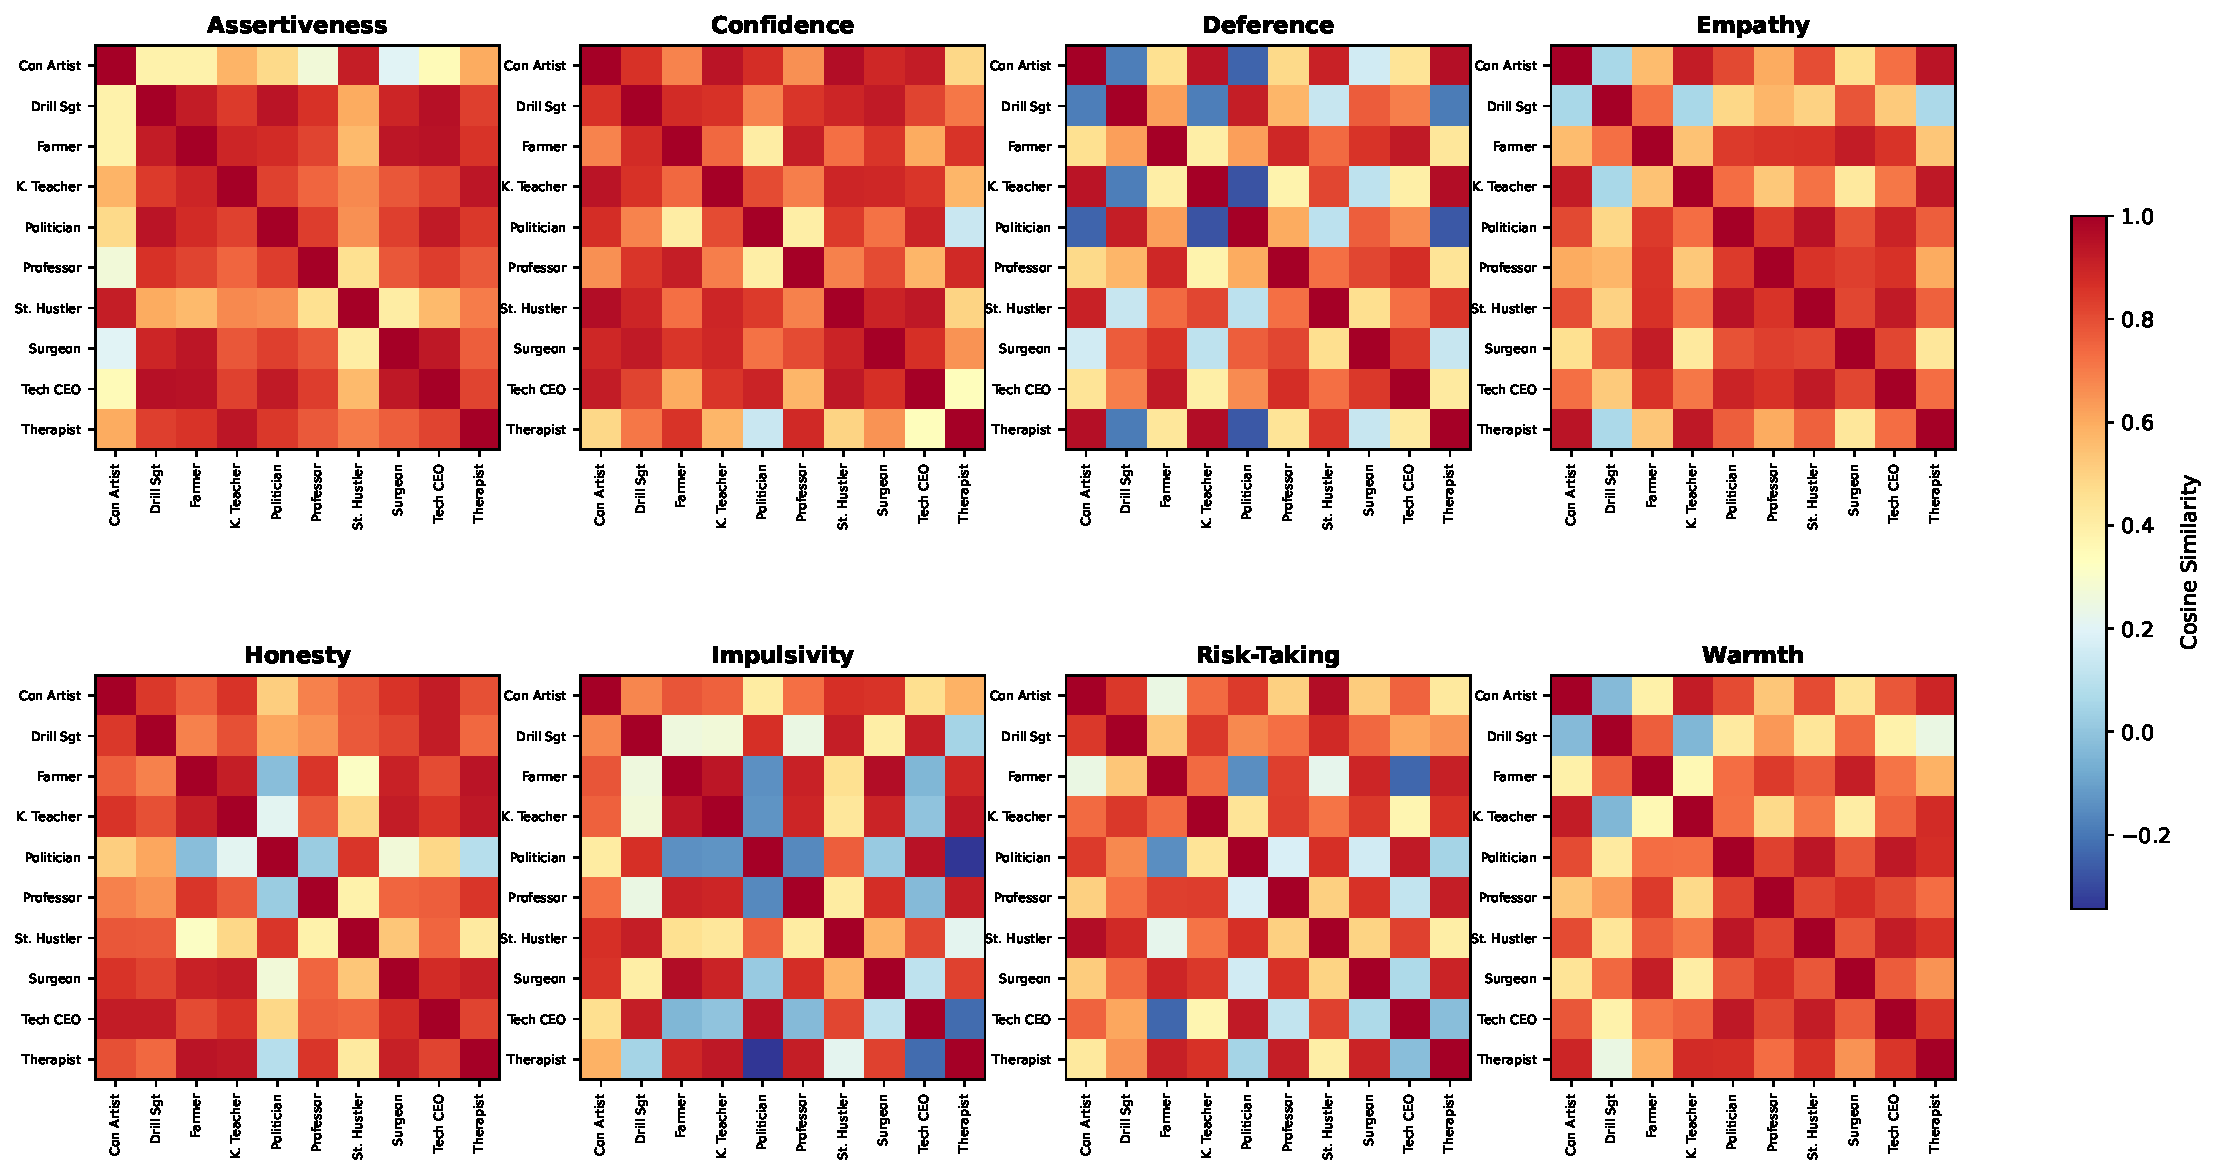
\includegraphics[width=0.88\linewidth]{figures/cosine_heatmaps.pdf}
\end{center}
\vspace{-3mm}
\end{posterblock}

% ══════════════════════════════════════════════════════════════
%  ROW 3: SHARED VARIANCE + SELF VS CROSS
% ══════════════════════════════════════════════════════════════
\noindent
\begin{minipage}[t]{0.485\textwidth}
\begin{posterblock}[equal height group=row3]{Shared vs Persona-Specific Variance}
\begin{center}
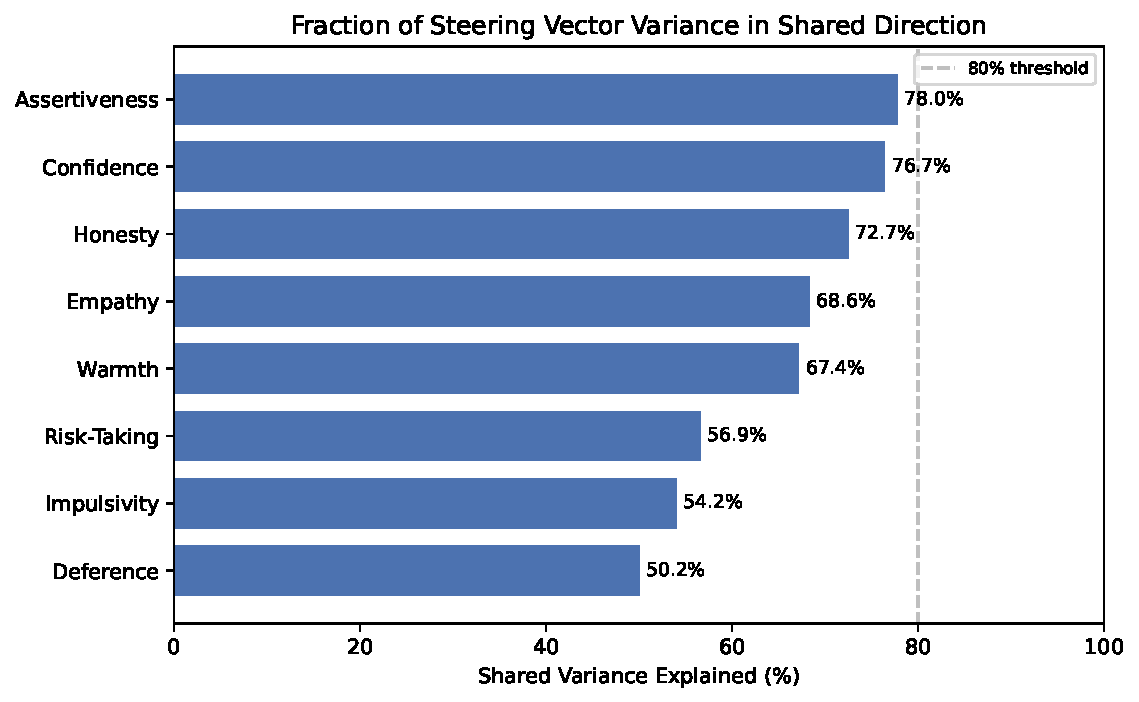
\includegraphics[width=0.88\linewidth]{figures/shared_variance.pdf}
\end{center}
% \vspace{-7mm}
\bodysize
No trait exceeds 80\% shared variance---all encode substantial persona-specific signal. Deference and impulsivity are most persona-conditioned (${\sim}50$\%).
\end{posterblock}
\end{minipage}\hfill
\begin{minipage}[t]{0.505\textwidth}
\begin{posterblock}[equal height group=row3]{Training Trajectory: OLMo-2 7B}
\begin{center}
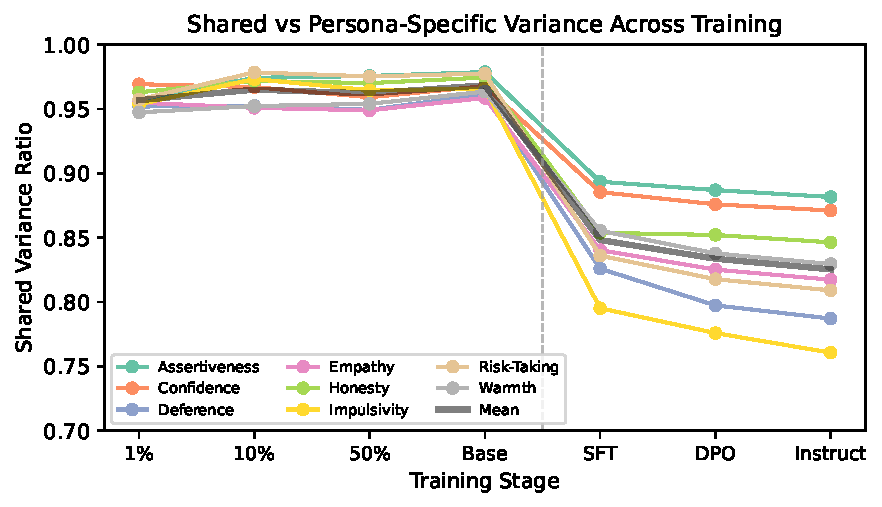
\includegraphics[width=0.88\linewidth]{figures/variance_trajectory.pdf}
\end{center}
% \vspace{-1mm}
\bodysize
Shared variance ratio across training stages (OLMo-2 7B). Persona-specific structure emerges at SFT/DPO---pretraining checkpoints show near-uniform vectors regardless of persona.
\end{posterblock}
\end{minipage}

% ══════════════════════════════════════════════════════════════
%  ROW 4: OBSERVATIONS + IMPLICATIONS + NEXT STEPS (stretch to fill)
% ══════════════════════════════════════════════════════════════

% Measure remaining space and define a stretched posterblock
\newlength{\remainingheight}
\setlength{\remainingheight}{\dimexpr\textheight-\pagetotal-22mm\relax}

\noindent
\begin{minipage}[t][\remainingheight]{0.32\textwidth}
\begin{posterblock}[equal height group=row4]{Key Observations}
\smallbody
\begin{itemize}[leftmargin=4mm, itemsep=3pt, labelsep=2mm, topsep=0pt]
    \item[\color{eracrimson}\textbullet] \textbf{Same trait, different vector}---persona identity reshapes encoding.
    \item[\color{eracrimson}\textbullet] \textbf{RLHF collapses diversity:} honesty shows high cross-persona similarity.
    \item[\color{eracrimson}\textbullet] \textbf{Intuitive pairs align:} K.\ teacher $\approx$ therapist on empathy.
    \item[\color{eracrimson}\textbullet] \textbf{Source ``residues'':} cross-steering leaks source biases into target.
\end{itemize}
\vfill
\end{posterblock}
\end{minipage}\hfill
\begin{minipage}[t][\remainingheight]{0.34\textwidth}
\begin{posterblock}[equal height group=row4]{Implications for Safety}
\smallbody
Safety work assumes vectors are \textbf{model-global}---one sycophancy vector works everywhere.

\smallskip
Our results challenge this: \textbf{persona-specific representations} mean a single intervention may not generalise across deployment contexts.

\smallskip
{\color{eracrimson}\textbf{Theory of change:}} Safety teams may need \textbf{persona-aware interventions} rather than one-size-fits-all vectors.
\vfill
\end{posterblock}
\end{minipage}\hfill
\begin{minipage}[t][\remainingheight]{0.32\textwidth}
\begin{posterblock}[equal height group=row4]{Next Steps \& References}
\smallbody
\begin{itemize}[leftmargin=4mm, itemsep=2pt, labelsep=2mm, topsep=0pt]
    \item[\color{eracrimson}\textbullet] Track across character training
    \item[\color{eracrimson}\textbullet] Safety traits: sycophancy, refusal
    \item[\color{eracrimson}\textbullet] Trait coupling (side-effects)
    \item[\color{eracrimson}\textbullet] More models (Llama, pre-instruct models)
\end{itemize}
\vfill
{\color{eracrimson}\rule{\linewidth}{0.5pt}}
\vspace{1mm}
{\captionsize
Chen et al.\ (2025). \emph{Persona Vectors.} arXiv:2507.21509.\par\smallskip
Lu et al.\ (2026). \emph{The Assistant Axis.} arXiv:2601.10387.\par
}
\end{posterblock}
\end{minipage}

% ══════════════════════════════════════════════════════════════
%  FOOTER
% ══════════════════════════════════════════════════════════════
\footnotetext{\fontsize{16}{21}\selectfont We also extracted vectors using an \emph{instruction-variant} method (opposing system-prompt instructions over shared questions). The key finding unique to that method: honesty converges to high shared variance across personas, consistent with RLHF collapsing representational diversity for heavily optimised traits.}

\end{document}
